\documentclass[a4paper,12pt]{article}

% Packages
\usepackage[utf8]{inputenc}
\usepackage[T1]{fontenc}
\usepackage{amsmath}
\usepackage{amssymb}
\usepackage{graphicx}
\usepackage{hyperref}
\usepackage{parskip}
\usepackage{animate}
\usepackage{comment}
\usepackage{subcaption}
\usepackage{geometry}
\geometry{margin=1in}

% Title and Author
\title{Flow Matching}
\author{Samy Braik}
\date{\today}

\begin{document}

\maketitle

We start by defining a probability density path \(p:[0,1]\times\mathbb{R}^d\rightarrow\mathbb{R}^d\) meaning that for each time \(t\), \(p_t\) is density function i.e. \(\int p_t(x)dx=1\).\\
A simple example of such a path is a path \(p\) interpolating two density \(p_0\) and \(p_1\) with \(p_t=tp_1+(1-t)p_0\)

\begin{comment}
\begin{figure}[h]
    \centering
    \animategraphics[autoplay,loop,width=1\linewidth]{10}{frame_}{000}{019}
    \caption{Probability path interpolating $\mathcal{N}(0,0.2)$ and $\mathcal{U}([0,1])$}
    \label{fig:interpolated_density}
\end{figure}
\end{comment}

\begin{figure}[htbp]
    \centering
    \begin{subfigure}[b]{0.45\textwidth}
      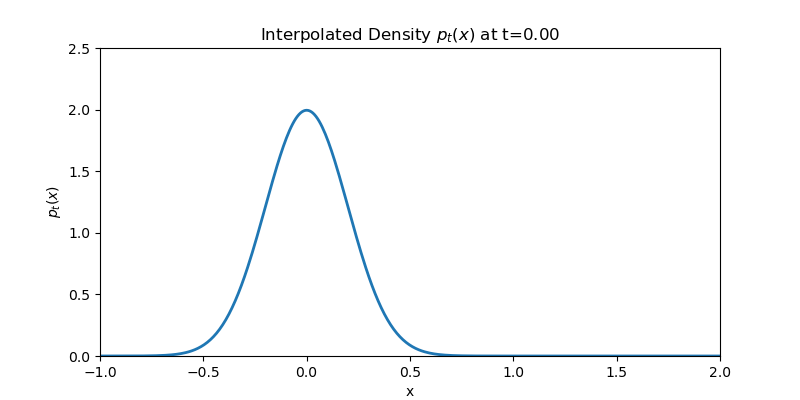
\includegraphics[width=\linewidth]{frames/frame_1.png}
      \caption{}
    \end{subfigure}
    \hfill
    \begin{subfigure}[b]{0.45\textwidth}
      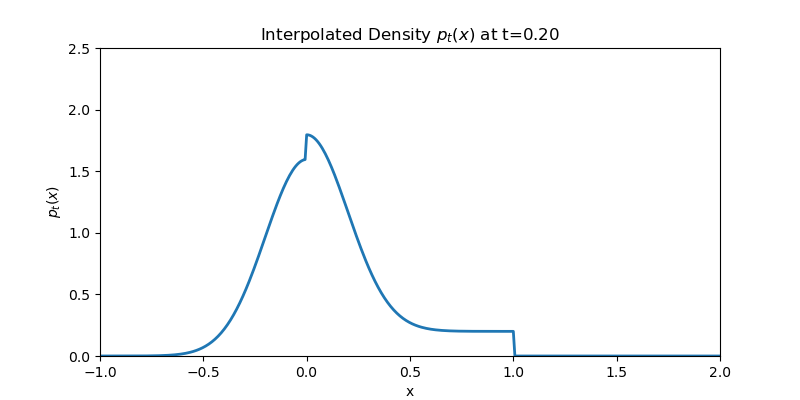
\includegraphics[width=\linewidth]{frames/frame_2.png}
      \caption{}
    \end{subfigure}
    \par\medskip
    \begin{subfigure}[b]{0.45\textwidth}
      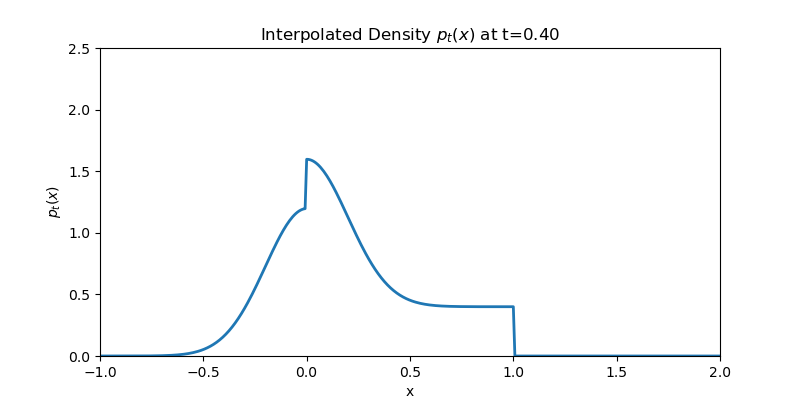
\includegraphics[width=\linewidth]{frames/frame_3.png}
      \caption{}
    \end{subfigure}
    \hfill
    \begin{subfigure}[b]{0.45\textwidth}
      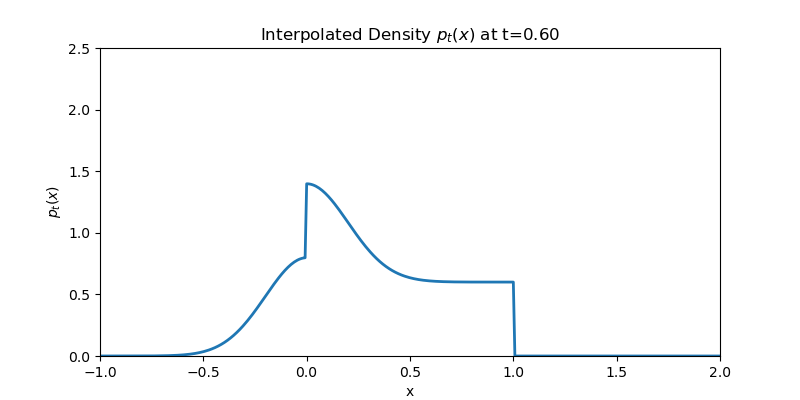
\includegraphics[width=\linewidth]{frames/frame_4.png}
      \caption{}
    \end{subfigure}
    \par\medskip
    \begin{subfigure}[b]{0.45\textwidth}
      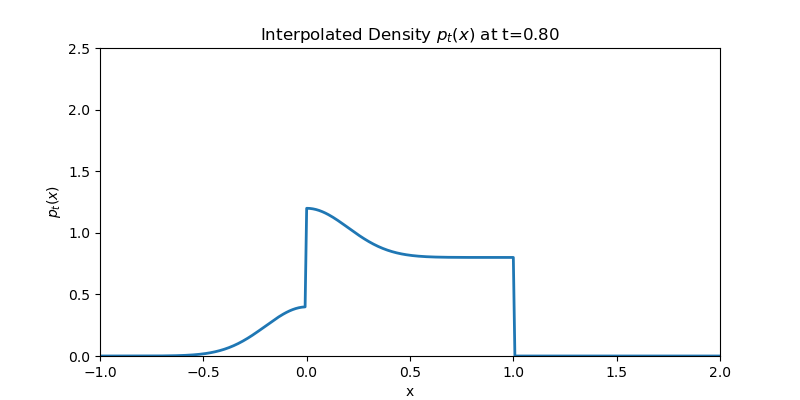
\includegraphics[width=\linewidth]{frames/frame_5.png}
      \caption{}
    \end{subfigure}
    \hfill
    \begin{subfigure}[b]{0.45\textwidth}
      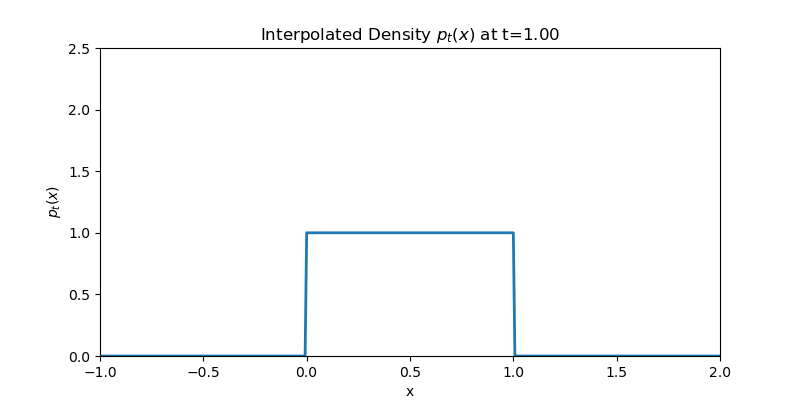
\includegraphics[width=\linewidth]{frames/frame_6.png}
      \caption{}
    \end{subfigure}
    \caption{A probability path interpolating $\mathcal{N}(0,0.2)$ and $\mathcal{U}([0,1])$}
    \label{fig:interpolated_density}
\end{figure}

\newpage

Next we introduce a core object, a time dependant vector field \(v:[0,1]\times \mathbb{R}^d\rightarrow\mathbb{R}^d\) which can be used to construct a map \(\phi:[0,1]\times\mathbb{R}^d\rightarrow\mathbb{R}^d\), called a flow, by the following ODE
\begin{align}
    \frac{d}{dt}\phi_t(x)&=v_t(\phi_t(x))\\
    \quad \phi_0(x)&=x \nonumber
\end{align}  
The link between the flow and the probability path is given by the change of variables formula 
\begin{align}
    p_t(x)=q(\phi_t^{-1}(x))\det \left[\frac{\partial\phi_t^{-1}}{\partial x}(x)\right]
\end{align}

\bibliographystyle{plain}
\bibliography{references}

\end{document}